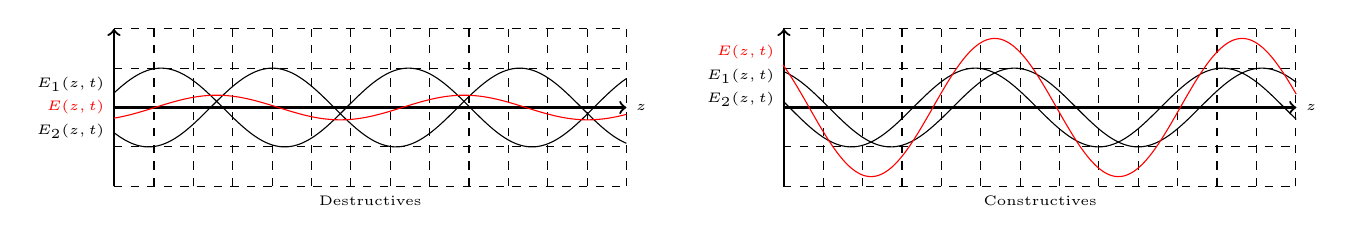
\begin{tikzpicture}
	
	%%% Grilles %%%
	
	\draw [dashed,step=0.5] (-2.39*pi,-1) grid (-1,1);
	\draw [dashed,step=0.5] (0.99,-1) grid (2.39*pi,1);
	
	%%% Axes %%%
	
	\draw[->,thick] (-2.39*pi,0) -- (-1,0);
	\draw[->,thick] (1,0) -- (2.39*pi,0);
	\draw[->,thick] (-2.39*pi,-1) -- (-2.39*pi,1);
	\draw[->,thick] (1,-1) -- (1,1);
	
	\draw (-1,0) node[anchor=west]{\tiny{$z$}};
	\draw (2.39*pi,0) node[anchor=west]{\tiny{$z$}};
	
	%%% Fonctions %%%
	
	\draw [domain=-2.39*pi:-1][samples=200]
	plot (\x,{sin(\x*2 r)*0.5});
	\draw [domain=-2.39*pi:-1][samples=200]
	plot (\x,{sin(deg(\x*2 + 0.9*pi))*0.5});
	\draw [domain=-2.39*pi:-1,color=red][samples=200]
	plot (\x,{sin(deg(\x*2 + 0.9*pi))*0.5+sin(\x*2 r)*0.5});
	
	\draw [domain=0.99:2.39*pi][samples=200]
	plot (\x,{sin(\x*2 r)*0.5});
	\draw [domain=0.99:2.39*pi][samples=200]
	plot (\x,{sin(deg(\x*2 +1))*0.5});
	\draw [domain=0.99:2.39*pi,color=red][samples=200]
	plot (\x,{sin(deg(\x*2 +1))*0.5+sin(\x*2 r)*0.5});
	
	%%% Labels %%%
	
	\draw (-2.39*pi*0.5-0.5,-1) node[anchor=north]{\tiny{Destructives}};
	\draw (2.39*pi*0.5+0.5,-1) node[anchor=north]{\tiny{Constructives}};
	
	\draw (-2.39*pi,0.3) node[anchor=east] {\tiny{$E_1(z,t)$}};
	\draw (-2.39*pi,-0.3) node[anchor=east] {\tiny{$E_2(z,t)$}};
	\draw (-2.39*pi,0) node[anchor=east,color=red]
	{\tiny{$E(z,t)$}};
	
	\draw (1,0.4) node[anchor=east] {\tiny{$E_1(z,t)$}};
	\draw (1,0.1) node[anchor=east] {\tiny{$E_2(z,t)$}};
	\draw (1,0.7) node[anchor=east,color=red]
	{\tiny{$E(z,t)$}};
	
\end{tikzpicture}